\chapter{Grundlagen} \label{ch:background}
Das Ziel von \ac{bi} ist es, aus operativen und externen Daten Informationen und aus diesem Wissen zu gewinnen. Damit ist es ein wertvolles Werkzeug zur Entscheidungshilfe und Planung. Prozesse zur Beschaffung, Transformation, Aufbereitung, Speicherung und Analyse von Daten, aber auch die Qualitätssicherung, sind Bestandteile eines BI-Systems \cite{muller_business_2013}. Ein BI-System kann in vier oder fünf grundlegende Bestandteile aufgeteilt werden. Die \textit{Datenversorgung} ist zuständig für den Zugriff auf verschiedene Datenquellen. Dabei können die Daten transformiert, aggregiert, bereinigt und auf Plausibilität geprüft werden. Die Speicherung der Daten fällt unter das \textit{Datenmanagement}. Anwendungen zur Aufbereitung und Darstellung dieser Daten gehören zu den \textit{BI-Anwendungen}. Im \textit{Metadatenmanagement}, werden relevante Metadaten, wie Zugriffsrechte oder Informationen zu dem Quellsystem verwaltet \cite{kemper_bi-glossar_2008}. Beim \textit{Warehouse Management} handelt es sich um die Verwaltung und Wartung der gesamten BI-Infrastruktur \cite{grunwald_business_2009}. Dazu zählt unter anderem die Überwachung der Systemauslastung und das Installieren von Softwareupdates. Das {Metadatenmanagement} wird nicht immer als eigener Bestandteil angesehen, sondern häufig als Teil des {Warehouse Managements} \cite{humm_architektur_2005}. So wird das {Metadatenmanagement} auch im Folgenden betrachtet.

\section{Verwandte Arbeiten} \label{ch:verwandteArbeiten}
\textit{...}

\section{Beschreibung der aktuellen on-premise BI-Architektur} \label{sec:grundlagen:onpremiseBI}
Die Ausgangslage für die Migration ist ein on-premise betriebenes BI~=System. Dieses ist in der \textit{Hub~=and~=Spoke-Architektur} aufgebaut. Diese gängige Architektur beschreibt die Verwendung eines zentralen Datenspeicherorts (Hub) und darauf aufbauenden, für bestimmte Auswertungen oder Anwendungen optimierte, Datenspeicher (Spokes) \cite{kemper_bi-glossar_2008}. Die Daten aus dem Hub werden also weiterverarbeitet und in den spezialisierten Spokes abgelegt. Abbildung~\ref{fig:aktuelle_onpremise_bi_architektur} zeigt die aktuelle BI~=Architektur, aufgeteilt nach funktionalen Bereichen.
\begin{figure}[htbp]
 \centering
 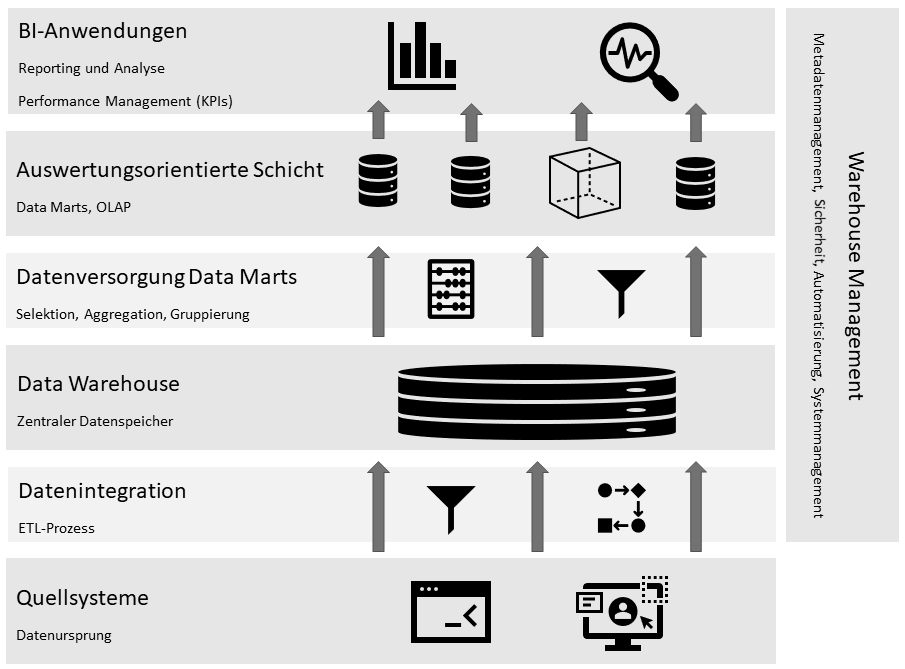
\includegraphics[width=\textwidth]{gfx/aktuelle_onpremise_bi_architektur.png}
 \caption{Aktuelle Architektur des on-premise BI-Systems und Ausgangslage für die Migration in die Cloud \cite{grunwald_business_2009}\cite{humm_architektur_2005}}
\label{fig:aktuelle_onpremise_bi_architektur}
\end{figure}
Die einzelnen Schichten werden im Folgenden erläutert \cite{grunwald_business_2009}\cite{kemper_bi-glossar_2008}\cite{humm_architektur_2005}:
\begin{itemize}
\item \textbf{Quellsysteme} sind der Ursprung aller Daten des BI-Systems. Es kann sich hierbei um interne, sowie externe Quellen handeln. Externe Daten könnten beispielsweise von Marktforschungs- oder Partnerunternehmen stammen. Aktuell sind nur interne Datenquellen angeschlossen. Darunter zum Beispiel die Projektmanagement-Software Jira und das Codeanalyse-Tool SonarQube.
\item Die \textbf{Datenintegration}(\ac{etl}) ist die Schnittstelle zwischen dem \ac{dwh} und den Quellsystemen. Der \acs{etl}-Prozess beginnt mit dem Extrahieren von operativen Daten aus einem Quellsystem. Darauf folgt eine Transformation, bei der die Daten an syntaktische Anforderungen angepasst werden und semantische Fehler, wenn möglich, behoben werden. Abschließend werden die Daten in das \ac{dwh} zur Speicherung geladen. Für den \acs{etl}-Prozess werden Funktionen von \textit{Microsofts SQL Server} und \textit{Powershell-Skripte} genutzt.
\item Das \textbf{Data Warehouse} ist der zentrale Speicherort. Hier werden die Daten strukturiert und langfristig abgelegt. Damit werden sie für weitere Verarbeitungsschritte und Auswertungen zur Verfügung gestellt. In diesem BI-System wird für das Data Warehouse das relationale Datenbankmanagementsystem \textit{Microsoft SQL Server} verwendet.
\item \textbf{Datenversorgung Data Marts}: Durch den Einsatz von SQL werden in dieser Schicht Bereich Daten selektiert, gruppiert und aggregiert. Das Ziel ist die Aufbereitung der Daten für die Data Marts.
\item \textbf{Auswertungsorientierte Schicht}: Data Marts beinhalten spezialisierte Ausschnitte der Daten aus dem \ac{dwh}, in einer für den Zugriff aus den BI-Anwendungen optimierten Form. Ziel ist es, dass für alle Anwendungsfälle eine effiziente Auswertung ermöglicht wird. Verschiedene Data Marts greifen beispielsweise auf die gleichen Daten mit unterschiedlichem Detailgrad und Selektionskriterien zu. Für komplexere Datenanalysen wird das Konzept des \textit{\ac{olap}} angewendet. Dieses soll es Nutzern ermöglichen, auch ohne technische Kenntnisse, Wissen aus dem \ac{dwh} oder den Data Marts zu extrahieren. Das kann durch die Bereitstellung von Ad-hoc-Reports geschehen, welche eine Benutzeroberfläche besitzen, über die mit einfachen Interaktionen flexible Analysen durchgeführt werden können. Dadurch sind keine Kenntnisse in einer Datenbankabfragesprache, wie SQL, notwendig. Die Grundlage für das \ac{olap} sind die sogenannten \ac{olap} Cubes. Unter diesen wird ein multidimensionaler Datenraum verstanden, bei dem die Dimensionen verschiedenen Kontexte, wie zum Beispiel Produkte, Kunden oder Zeit beschreiben. Sowohl die Data Marts als auch die \ac{olap} Cubes sind entweder als View auf das \ac{dwh} oder als eigenständige Datenbanktabelle realisiert.
\item \textbf{BI-Anwendungen} sind die Benutzerschnittstelle zum BI~=System. Hier erfolgen Auswertung und Präsentation. Im aktuellen BI~=System existieren drei Reporting-Anwendungen, die jeweils eine andere Management~=Ebene als Zielgruppe haben. Von den verschiedenen Arten an BI~=Anwendungen werden die Kategorien \textit{Reporting und Analyse} und \textit{Performance Management} abgedeckt. Bei der ersten Kategorie werden standardisierte Berichte in Form von Listen, Tabellen und Grafiken zur Verfügung gestellt. Beim {Performance Management} wird die Unternehmensleistung anhand von ausgewählten \acp{kpi} dargestellt und mit Zielwerten verglichen. Die vorhandenen BI-Anwendungen wurden mit einem internen Reporting~=Framework entwickelt, das auf dem Web~=Framework AngularJS und einer Java"-script Bibliothek zum Erstellen von Visualisierungen basiert.
\item Das \textbf{Warehouse Management} umfasst Aufgaben bezüglich Aufbau, Pflege und Betrieb des BI-Systems:
\begin{itemize}
\item \textit{Metadatenmanagement}. Verwaltung von Metadaten und Bereitstellung einer gemeinsamen Metadatenbasis für alle Komponenten im System.
\item \textit{Sicherheit}. Authentifizierung und Autorisierung von Benutzern.
\item \textit{Automatisierung}. Event- oder zeitbasierte Ausführung von Prozessen im \ac{dwh}. Zum Beispiel das Ausführen eines ETL-Prozesses zu einer festen Uhrzeit.
\item \textit{Systemmanagement}. Betrieb des \ac{dwh}s gewährleisten. Dazu gehört zum einen die Überwachung von Performance und Auslastung des Systems und zum anderen die Archivierung und Sicherung von Daten.
\end{itemize}
\end{itemize}

\section{Microsoft Azure Cloud} \label{sec:grundlagen:bi_in_der_cloud_mit_azure}

\subsection{Entscheidung für die Microsoft Azure Cloud} \label{subsec:grundlagen:azure:entscheidungFürAzure}
Microsoft Azure wird intern bereits für andere Anwendungsfälle genutzt und ist der einzige Cloud-Provider, der aktuell von der Software AG für die Speicherung und Verarbeitung von Unternehmensdaten zugelassen ist. Mit Microsoft bestehen bereits entsprechende Verträge und die notwendige Zustimmung vom Betriebsrat liegt vor. Die Verwendung eines anderen Cloud-Providers wäre theoretisch möglich, ist aber in der aktuellen Unternehmensstrategie nicht vorgesehen und würde damit einen deutlich größeren organisatorischen Aufwand bedeuten. Deswegen beschränkt sich diese Arbeit auf die Azure Cloud.

Neben den internen Gründen gibt es aber auch fachliche Argumente für die Wahl von Azure. Hier werden alle Vorteile der Cloud mit gleichzeitig hoher Flexibilität geboten. Die große Auswahl an unterstützten Betriebssystemen, Plattformen und Tools soll es den Kunden ermöglichen, nahezu alle gewünschten Technologien zu verwenden. Des Weiteren hat Microsoft auf der ganzen Welt verteilt Datenzentren und ist auf eine schnelle Disaster Recovery vorbereitet \cite{modi_azure_2020}. Für das hier verfolgt Ziel ist jedoch folgende Aussage aus \citetitle{modi_azure_2020} am wichtigsten "\textit{[...] it provides a host of interconnected services that can pass data among themselves. With such capabilities in place, data can be processed to generate meaningful knowledge and insights}" \cite{modi_azure_2020}. Die Azure Cloud bietet demnach einige Möglichkeiten für die Konstruktion einer BI-Infrastruktur.

\subsection{Business Intelligence in der Cloud} \label{subsec:grundlagen:azure:bi}
In der Cloud wird eine Vielzahl an Ressourcen, wie virtualisierte Hardware oder Dienste, zur Verfügung gestellt. Diese können dynamisch konfiguriert und skaliert werden, sodass immer die benötigte Leistung zur Verfügung steht. Microsoft Azure ist eine Sammlung an solchen Ressourcen, die sich aktuell in 22 Kategorien einteilen lassen. Manche Dienste können dabei zu mehreren Kategorien gehören. Für den Entwurf der neuen BI-Architektur werden Dienste aus den folgenden Kategorien in Betracht gezogen \cite{chilberto_building_2020}:
\begin{itemize}
\item \textbf{Integrations}~=Dienste können eingesetzt werden, um die Daten aus Cloud und on-premise Anwendungen zu laden.
\item \textbf{Datenbank}~=Dienste sind unter anderem relationale Datenbanken, wie Azure SQL, MySQL und PostgreSQL. Eine Alternative dazu ist die NoSQL-Datenbank Azure Cosmos DB, welche mehrere Datenmodelle unterstützt.
\item \textbf{Speicher}-Dienste sind in verschiedenen Ausprägungen vorhanden und können nach den individuellen Anforderungen ausgewählt werden. Ziel ist es, eine große Menge an Daten, die sowohl strukturiert als auch unstrukturiert sein kann, möglichst günstig abzuspeichern.
\item \textbf{Analyse}-Dienste helfen, die benötigten Erkenntnisse aus den Daten zu gewinnen.
\item \textbf{KI und Machine Learning} ermöglicht komplexere Analysen. Zum Beispiel können, basierend auf historischen Daten, Vorhersagen über die Zukunft getroffen werden. Diese können beispielsweise genutzt werden, um die zukünftige Entwicklung von KPIs abzuschätzen.
\item \textbf{Identitäts}-Dienste werden genutzt, um sicherzustellen, dass nur berechtigte Nutzer Zugriff auf Anwendungen und Daten erhalten.
\item \textbf{Netzwerk}-Dienste werden verwendet, um eine sichere Verbindung zwischen on-premise und Cloud Infrastruktur herzustellen.
\item \textbf{Sicherheit} ist ein wichtiges Kriterium für Cloud-Systeme. Azure stellt hierfür Dienste zur Überwachung der Datensicherheit und zum Erkennen von Sicherheitsrisiken bereit.
\item \textbf{Verwaltung und Governance} umfasst Dienste zur Automatisierung, sowie zur Verwaltung und Überwachung der Cloud-Ressourcen. Dazu gehört das Erstellen von Backups, sowie das Monitoring von Anwendungen, der Infrastruktur und den dadurch entstehenden Kosten.
\item \textbf{Migrations}-Dienste sollen beim Umstieg von on-premise zu Cloud Ressourcen unterstützen. Sie könnten zum Beispiel eingesetzt werden, um Daten aus dem bestehenden \ac{dwh} in eine Cloud Alternative zu übertragen.
\end{itemize}
Beim Vergleich der Azure Kategorien mit den funktionalen Schichten des on-premise BI-Systems decken die \textit{Integrations-Dienste} die Funktionalität der \textit{Datenintegration} ab. Das \ac{dwh} kann in Azure entweder mit den \textit{Datenbank-}, den \textit{Speicher-Diensten} oder einer Kombination von beiden ersetzt werden. Die \textit{Analyse-Dienste} entsprechen der \textit{auswertungsorientierten Schicht} und den \textit{BI-Anwendungen} des on-premise Systems. Zusätzlich neue Auswertungsmöglichkeiten bieten die Dienste aus \textit{KI und Machine Learning}. Die Kategorien \textit{Identität}, \textit{Netzwerk}, \textit{Sicherheit} und \textit{Verwaltung und Governance} sind vergleichbar mit dem \textit{Warehouse Management}.

\subsection{Dienste für Sicherheit und Datenschutz} \label{subsec:grundlagen:azure:sicherheitUndDatenschutz}
Neben den Azure Diensten zur Erfüllung der funktionalen Anforderungen, die erst in Abschnitt~\ref{sec:konzeption:evaAuswertung} festgelegt werden, sollen weitere Dienste für die Sicherheit und den Datenschutz beim Entwurf der neuen BI-Architektur berücksichtigt werden.

\subsubsection{Azure Policy} \label{subsec:grundlagen:azure:sicherheitUndDatenschutz:ap}
Mit \textit{Azure Policy} kann die Einhaltung bestimmter Compliance Anforderungen für alle Azure Ressourcen erzwungen werden. Dies wird für das System regelmäßig überprüft. Dazu werden zunächst die einzuhaltenden Parameter, wie beispielsweise der Serverstandort, festgelegt. So kann der Versuch eine Ressource zu erstellen, die gegen die festgelegten Compliance Standards verstößt, verhindert werden. Durch \textit{Azure Policy} kann also eine konsistente Einhaltung der Compliance im gesamten BI-System sichergestellt werden \cite{stefanovic_azure_2021}.

\subsubsection{Azure Key Vault} \label{subsec:grundlagen:azure:sicherheitUndDatenschutz:keyVault}
Der \textit{Azure Key Vault} ist ein sicherer Cloud-Speicherplatz für Schlüssel, Passwörter und Zertifikate. Dafür verfügt jedes Rechenzentrum über ein Hardware-Sicherheitsmodul, welches durch den Einsatz von verschiedenen Sensoren sowohl Hacking-Attacken als auch physische Zugriffsversuchen erkennen kann. In diesem Fall werden alle Passwörter automatisch von der Festplatte gelöscht. Deswegen liegt immer mindestens eine Kopie der Daten in einem anderen Rechenzentrum vor \cite{haunts_key_2019}.

\subsubsection{Azure Active Directory} \label{subsec:grundlagen:azure:sicherheitUndDatenschutz:aad}
\ac{aad} ist ein cloudbasierter Identitäts- und Zugangsverwaltungsdienst. Durch diesen können sich die Nutzer mit Benutzernamen und Passwort authentifizieren. Für eine erhöhte Sicherheit wird außerdem die Verwendung der inzwischen Standard gewordenen \ac{mfa} unterstützt.

\ac{aad} ermöglicht die Umsetzung von \ac{rbac}. Mit \ac{rbac} können die Zugriffsrechte einer Identität auf die Azure Ressourcen granular festgelegt werden \cite{stefanovic_azure_2021}.

%\subsubsection{Microsoft Defender for Cloud} \label{subsec:grundlagen:azure:sicherheitUndDatenschutz:asc}
% Der \textit{Microsoft Defender for Cloud} (ehemals Azure Security Center) soll einen Überblick über die Sicherheit der gesamten Infrastruktur geben. Dazu gibt es unter anderem ein Sicherheitsrating, das als Maßstab für die Bewertung der Systemsicherheit verwendet werden kann \cite{buchanan_azure_2022}.

\section{Migrationsstrategie} \label{sec:beschreibungMigrationsstrategie}
In der Literatur wird zwischen drei Migrationsstrategien unterschieden \cite{juan-verdejo_moving_2014}:
\begin{enumerate}
\item \textbf{Teilweise nach Fachbereichen}: Die Migration wird nur für einzelne Fachbereiche durchgeführt. Zum Beispiel wird das BI-System für den Kundensupport migriert, während das BI-System für den Vertrieb weiterhin on-premise betrieben wird.
\item \textbf{Teilweise nach Schichten}: Es werden nicht alle funktionalen Schichten in die Cloud migriert. Aus Sicherheitsbedenken könnte beispielsweise die Speicherung von Daten weiterhin on-premise erfolgen, während die Datenanalysen und Auswertungen mit Cloud Ressourcen durchgeführt werden.
\item \textbf{Vollständig}: Das gesamte on~=premise BI~=System wird durch eine Cloud~=Lösung ersetzt.
\end{enumerate}
Für das bestehende BI-System soll die vollständige Migrationsstrategie angewendet werden. \textit{1.} wäre nicht sinnvoll, da für das gesamte BI-System nur ein Team zuständig ist. \textit{2.} wird hauptsächlich aus Sicherheitsgründen angewendet, führt dabei aber oft zu Performance Einbußen. Da die Sicherheit bereits ein wichtiges Kriterium der neuen BI~=Architektur ist, wird diese Strategie als nicht notwendig erachtet.

\section{Spezifikation der Anforderungen}
Die Anforderungen an die neue BI-Architektur werden in iterativen Meetings mit den Stakeholdern festgelegt. Eine besondere Herausforderung hierbei ist es, dass die Anforderungsanalyse unvoreingenommen durchgeführt wird. Die Anforderungen sollten weder aus der aktuellen BI-Lösung noch aus individuellen Lösungsideen abgeleitet werden. Stattdessen sollten sie sich auf die Essenz des Systems beziehen, also den geschäftlichen Grund für den Einsatz des BI-Systems \cite[vgl.][]{robertson_mastering_2013}.

Als Grundlage für die Anforderungsspezifikation wird eine aktuelle Version des \citetitle{robertson_volere_2020}\textit{s} \cite{robertson_volere_2020} verwendet. Dieses gibt eine grundlegende Struktur und Kategorisierung vor. Hier wird außerdem Wert darauf gelegt, dass beim Beschreiben einer Anforderung ein Testkriterium festgelegt wird. Dadurch werden die Anforderungen messbar und es kann später eindeutig festgestellt werden, ob sie erfüllt wurden. Abgesehen davon werden jedoch nur die Bestandteile der Vorlage übernommen, die für die Evaluation in Abschnitt~\ref{sec:evaluation} als relevant angesehen werden.

Weggelassen wurden Anforderungen an die Benutzerfreundlichkeit und kulturelle Anforderungen, weil für den Endnutzer Reports die einzige Schnittstelle zum BI-System sind. In dieser Arbeit steht jedoch die Architektur im Vordergrund, deswegen ist nur die grundsätzliche Möglichkeit, vielfältige Reports zu erstellen, wichtig. Es ist hier nicht vorgesehen, die Reports zu optimieren. Auch operative und umweltbezogene Anforderungen sind für die Evaluation nicht relevant, da kein Release geplant ist und alle Azure Dienste in einer vergleichbaren physikalischen Umgebung laufen.